\begin{figure}
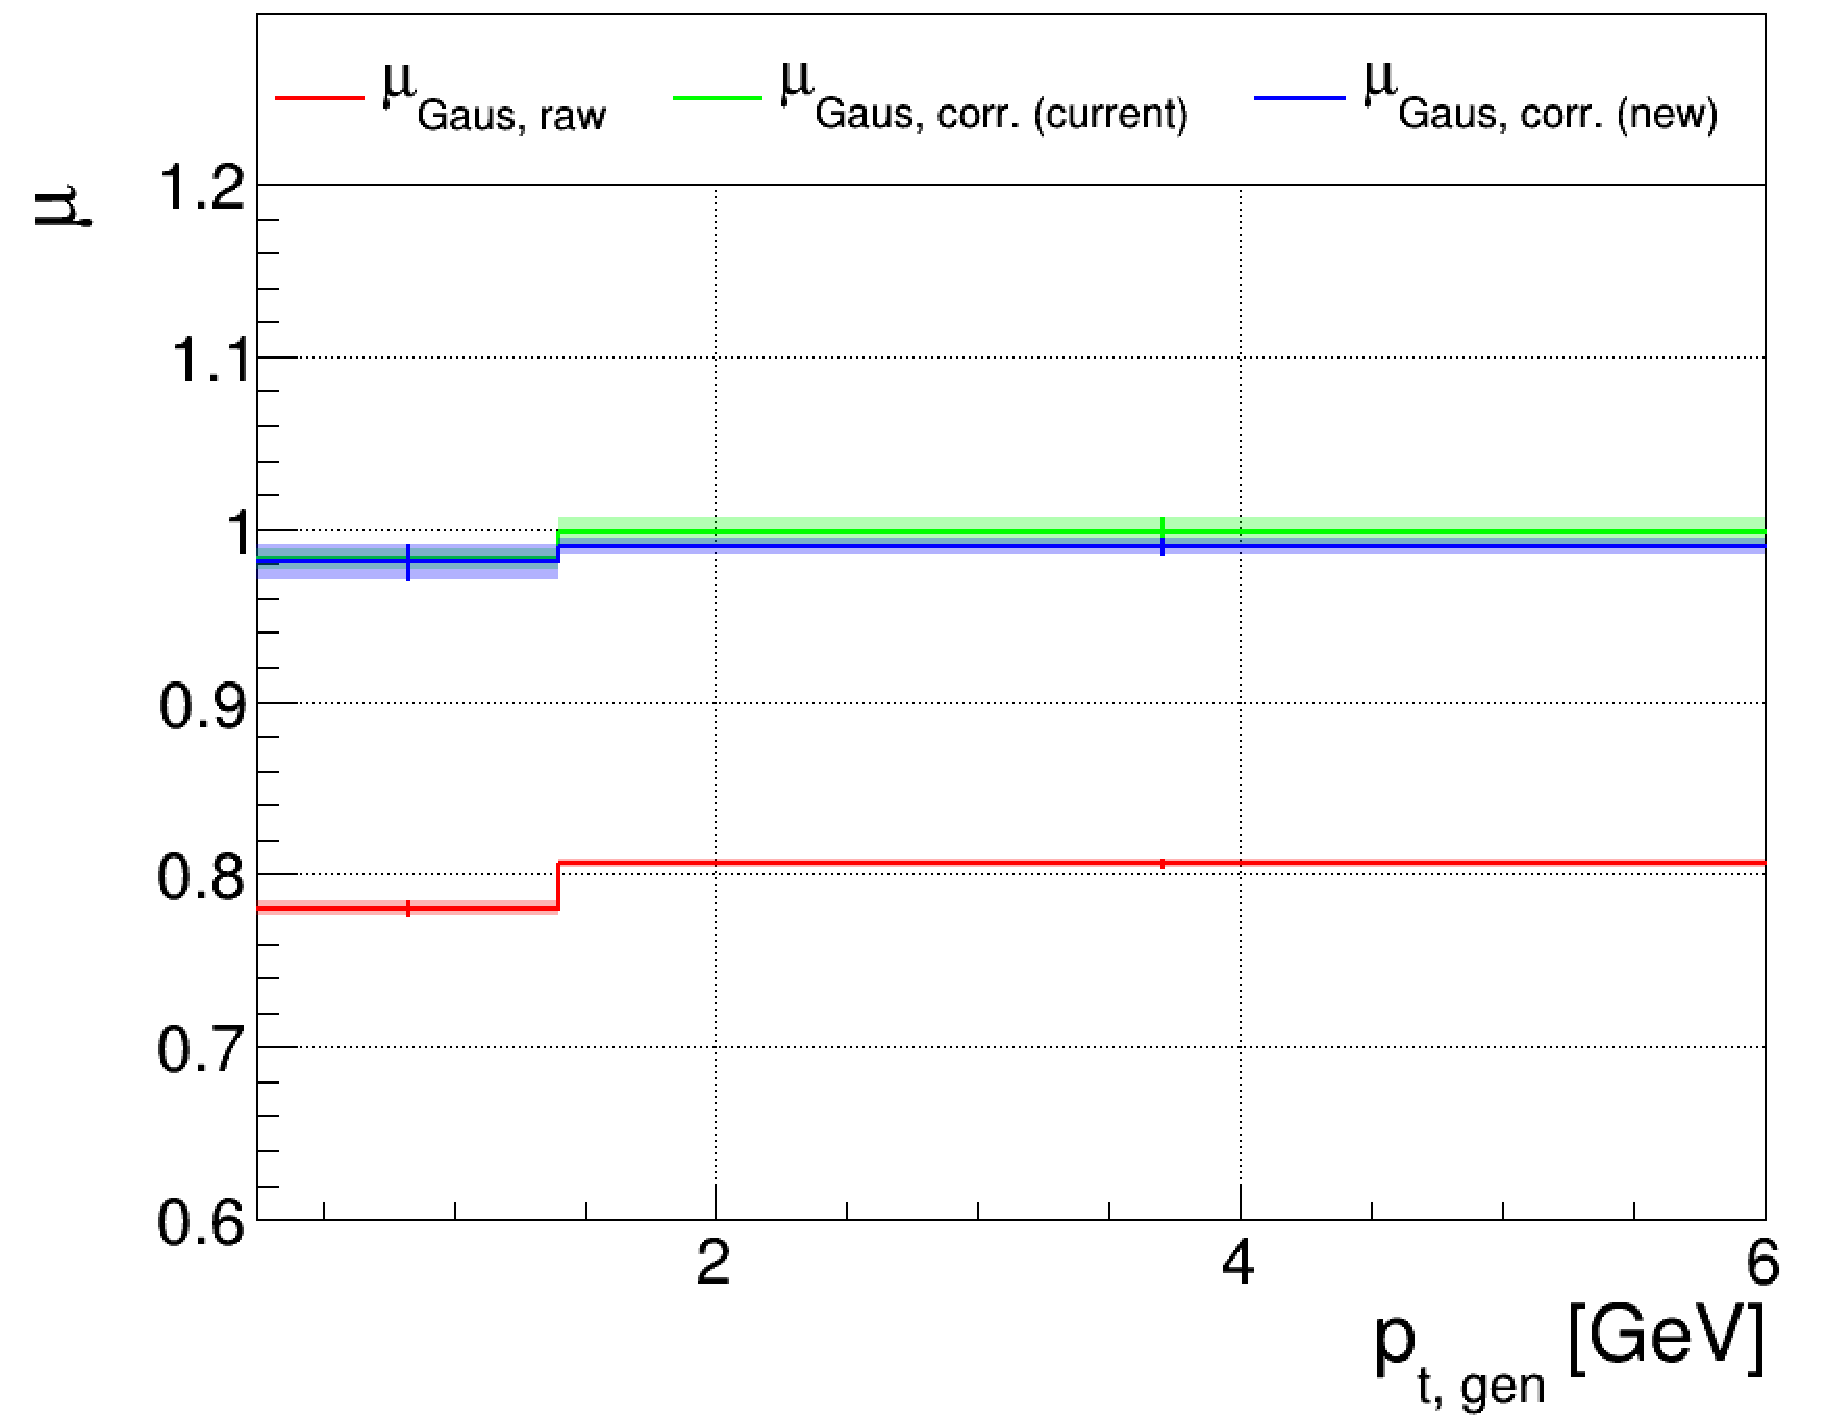
\includegraphics[width=0.495\textwidth]{./plots_pdf/ECAL_plots/plotsNoPU/EE/pdf/ZS/GENPT/EEZS_GENPT_0000_0006_MuOverBins.pdf}
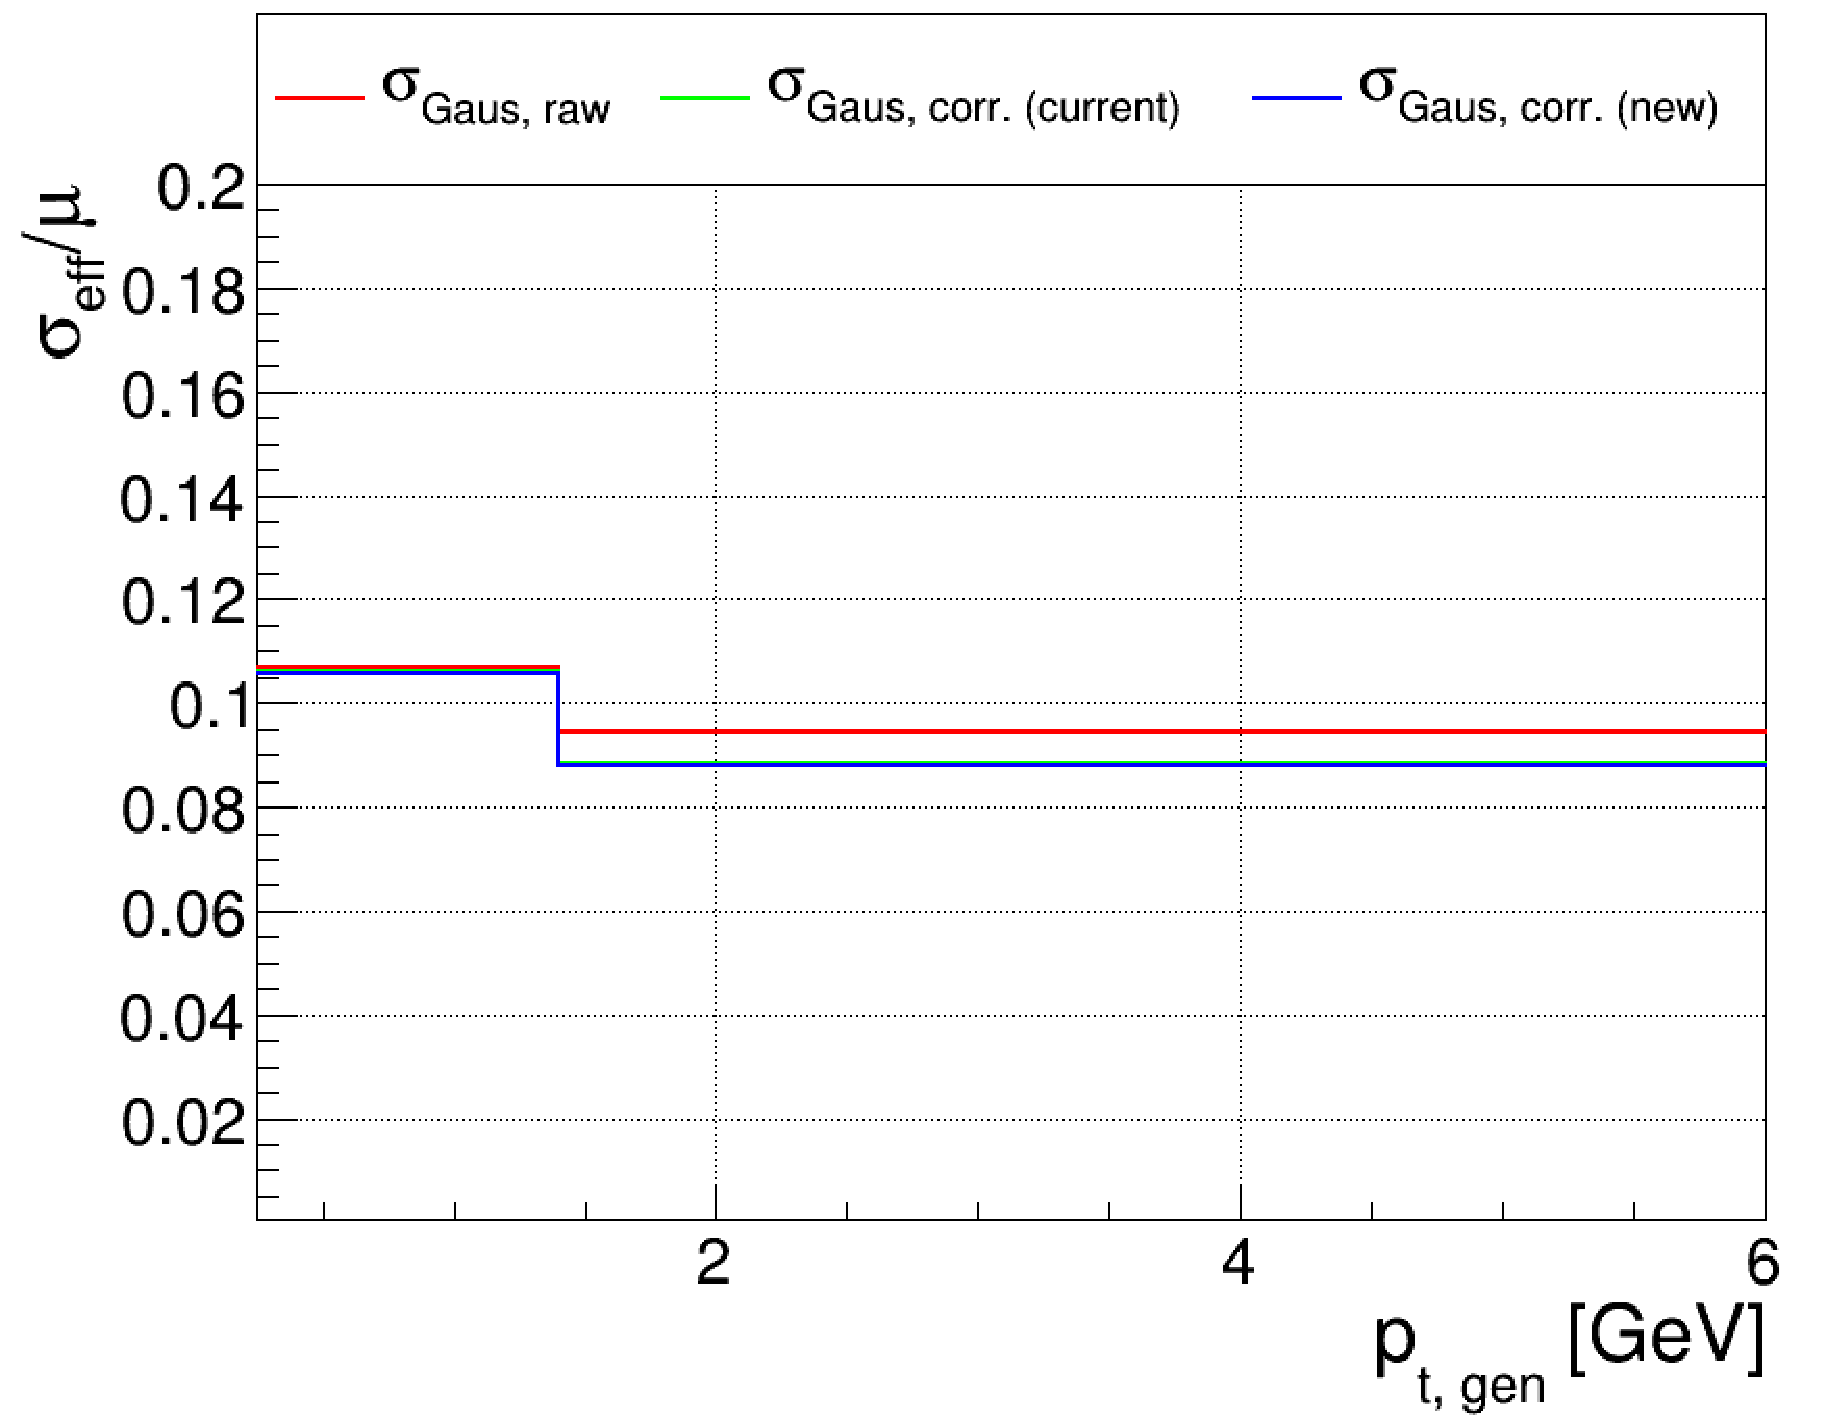
\includegraphics[width=0.495\textwidth]{./plots_pdf/ECAL_plots/plotsNoPU/EE/pdf/ZS/GENPT/EEZS_GENPT_0000_0006_EffSigmaOverBins.pdf}

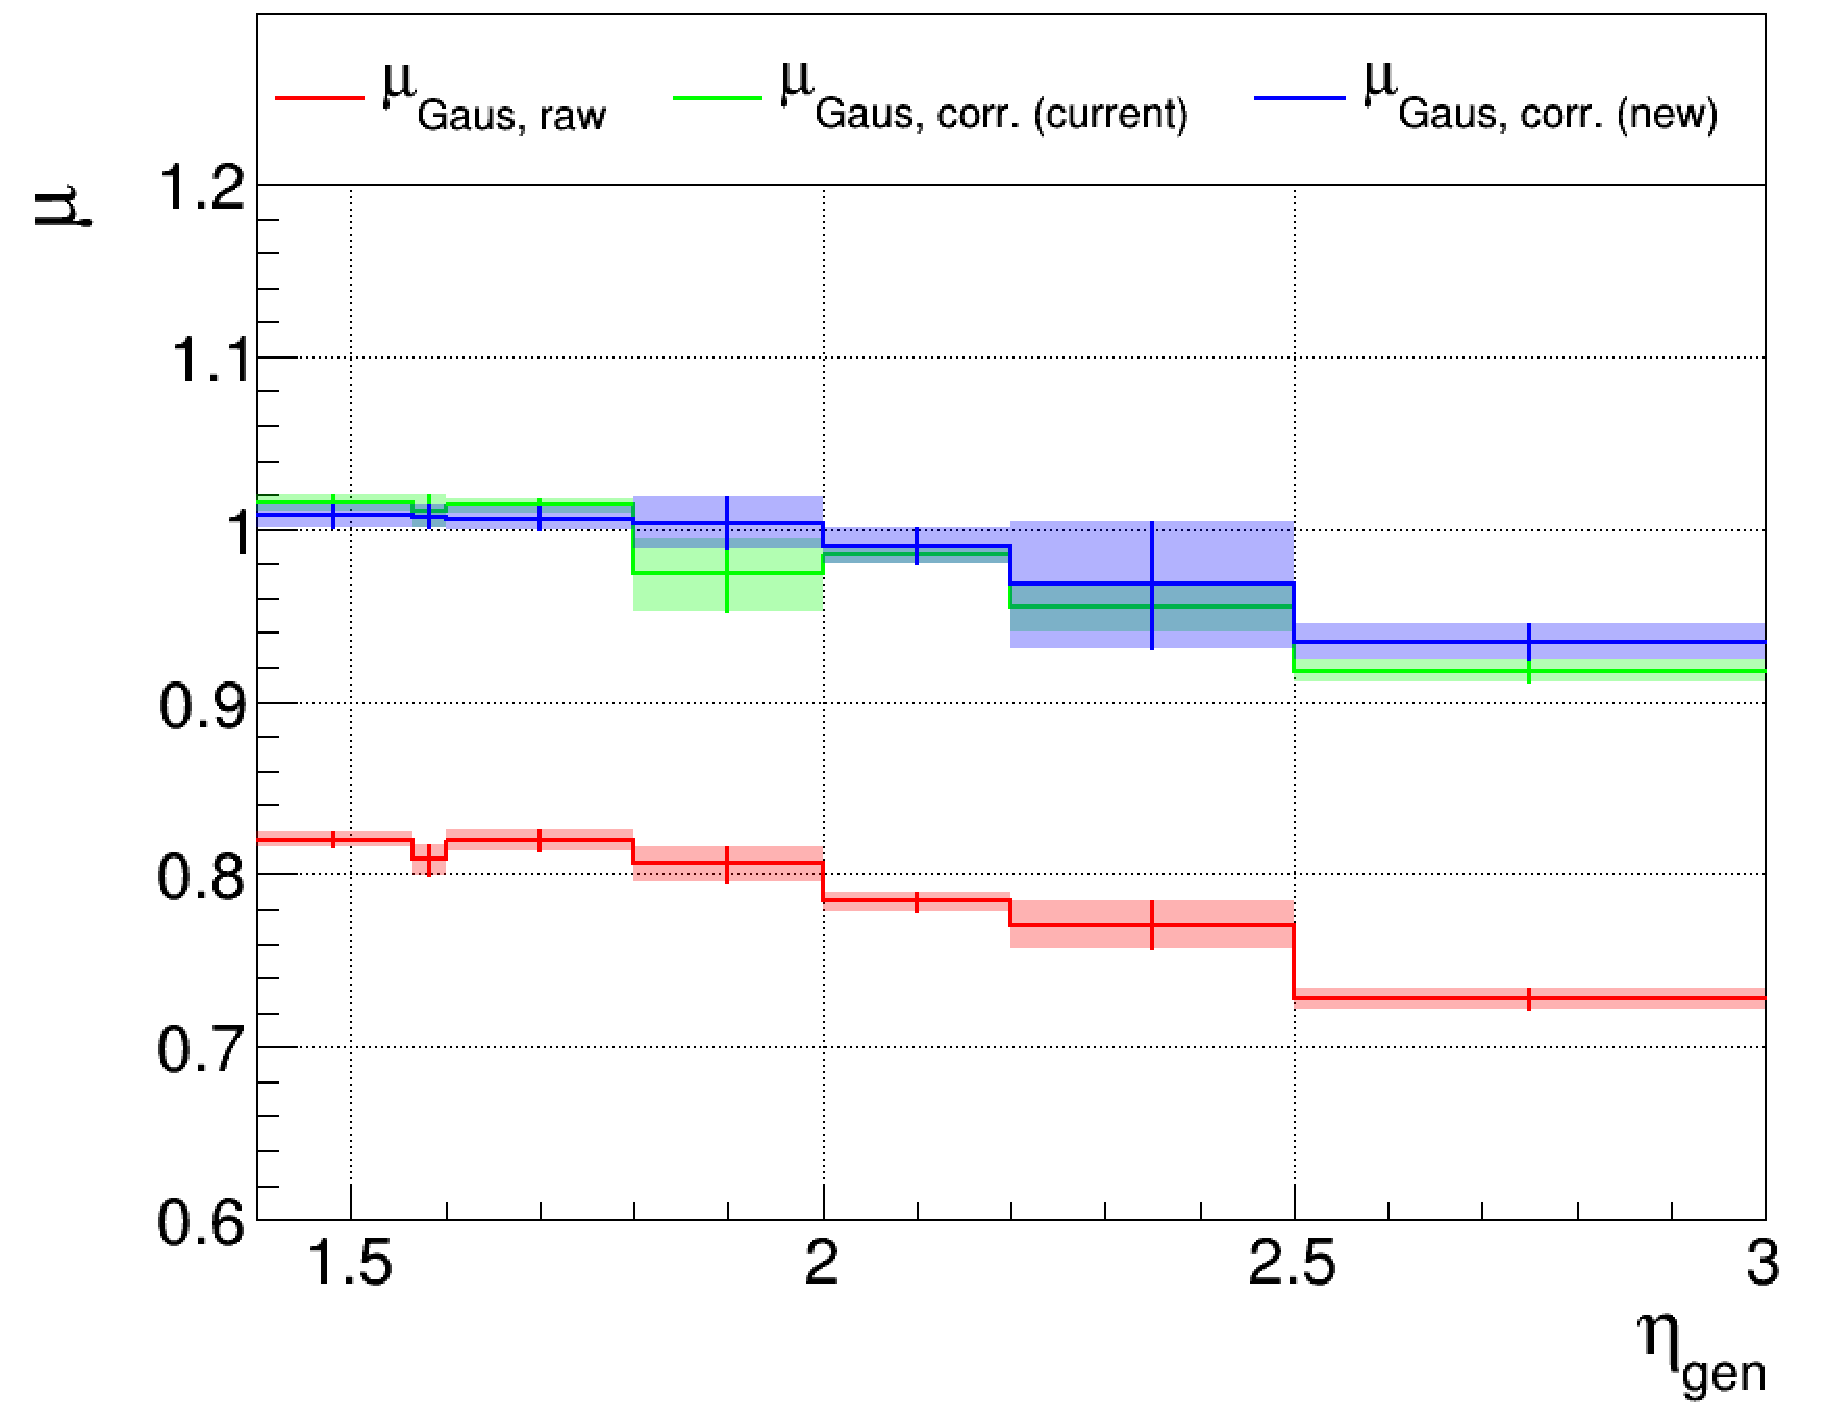
\includegraphics[width=0.495\textwidth]{./plots_pdf/ECAL_plots/plotsNoPU/EE/pdf/ZS/GENETA/EEZS_GENETA_0000_0006_MuOverBins.pdf}
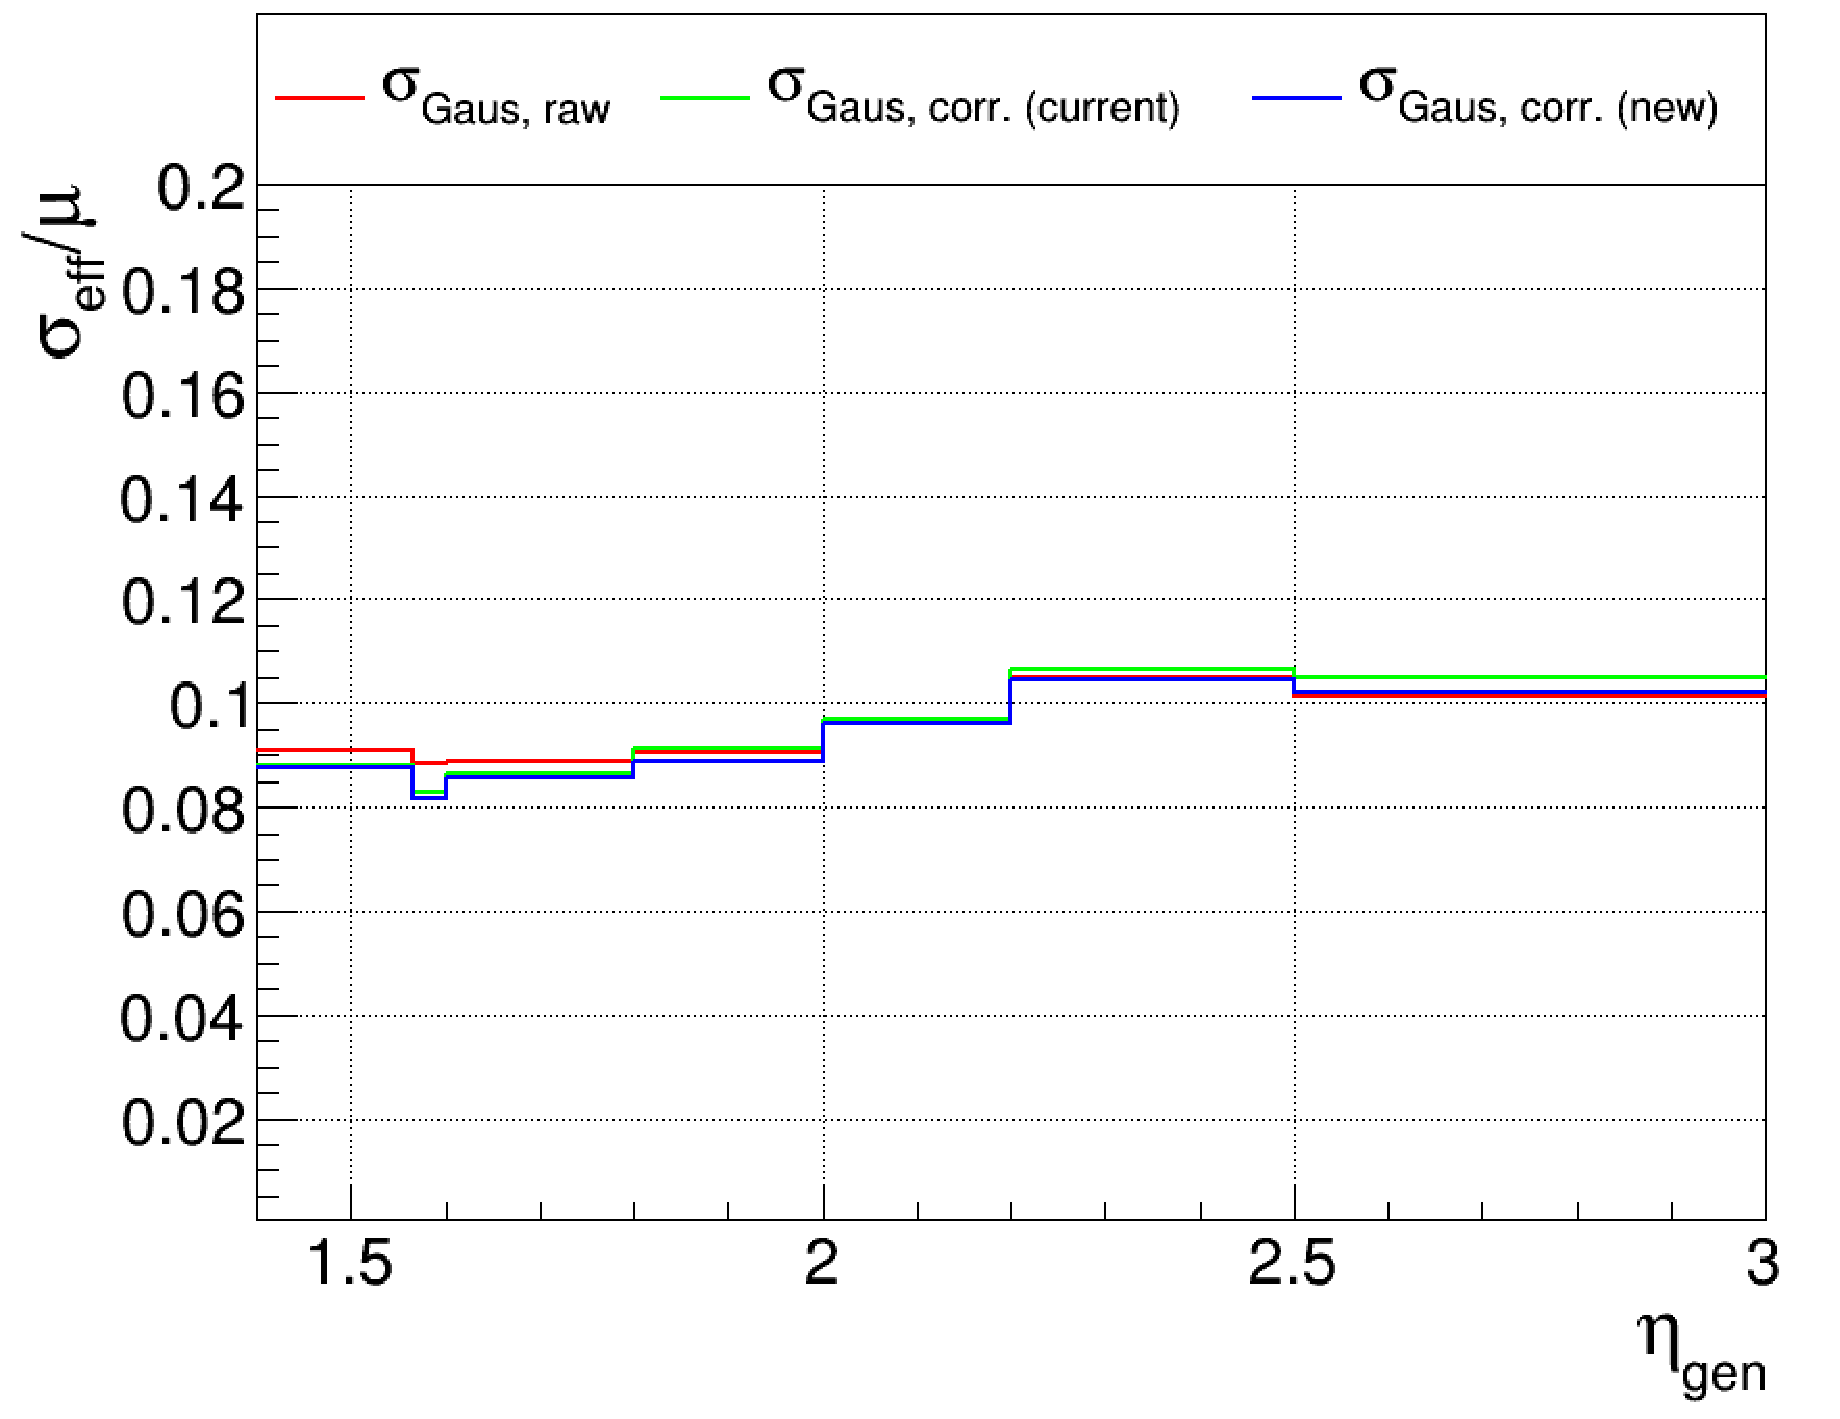
\includegraphics[width=0.495\textwidth]{./plots_pdf/ECAL_plots/plotsNoPU/EE/pdf/ZS/GENETA/EEZS_GENETA_0000_0006_EffSigmaOverBins.pdf}
\caption[$\mu$ ($\sigma_\mathrm{eff}$) vs \pt of PF ECAL cluster - EE ZS readout NoPU scenario]{Mean response (resolution) defined by Raw PF ECAL clusters (red), the calibration derived earlier in Ru\
n3 based on 126X (green), and the new correction from 2024 simulation sample based on 133X (blue).\pt 0--6\GeV in EE region ZS Readout NOPU scenario.}
\end{figure}

%% %\begin{figure}
%% 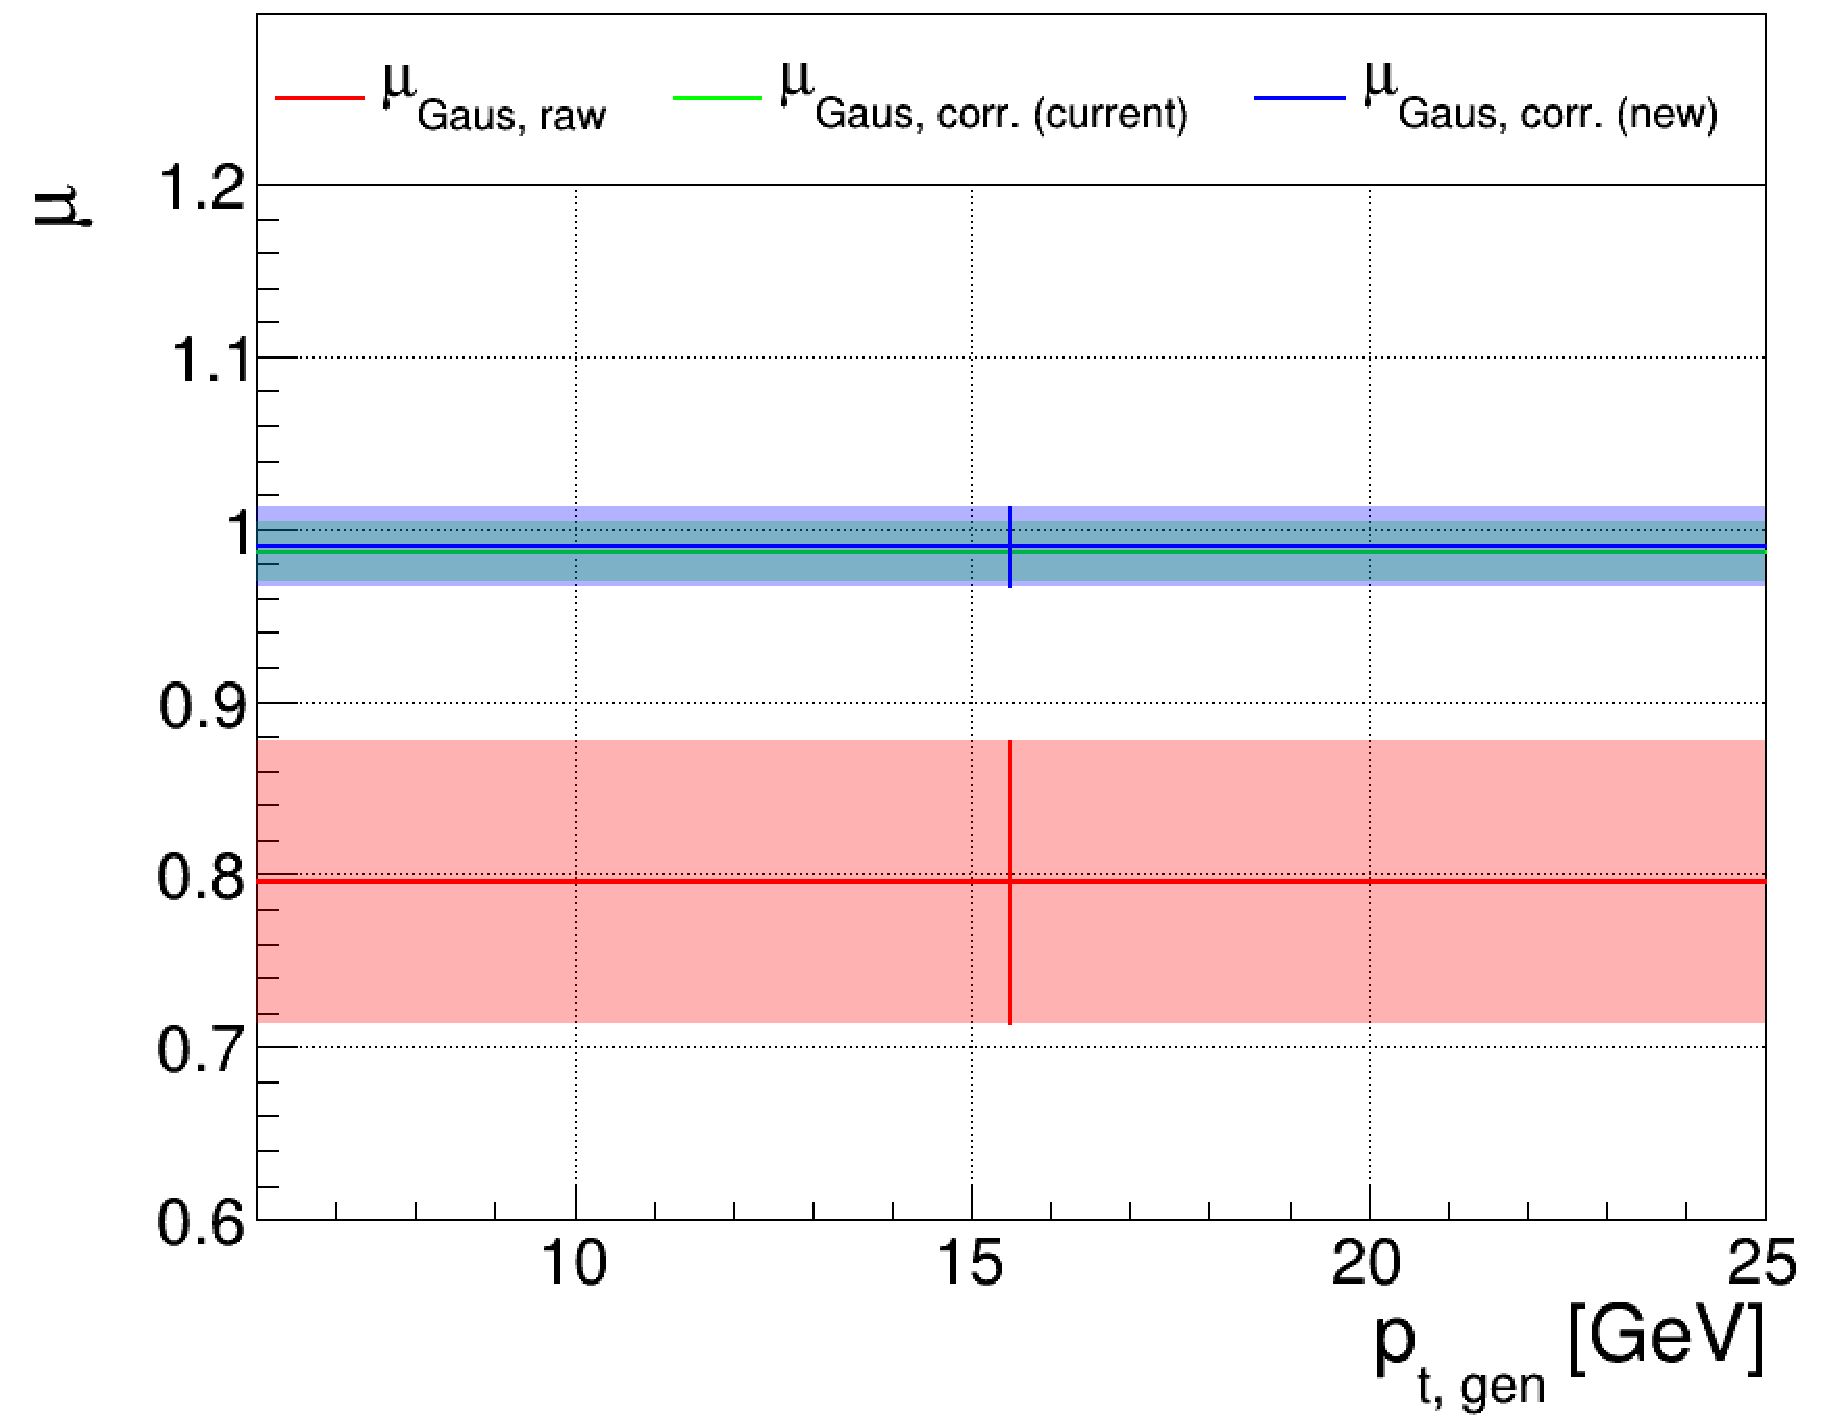
\includegraphics[width=0.495\textwidth]{./plots_pdf/ECAL_plots/plotsNoPU/EE/pdf/ZS/GENPT/EEZS_GENPT_0006_0025_MuOverBins.pdf}
%% 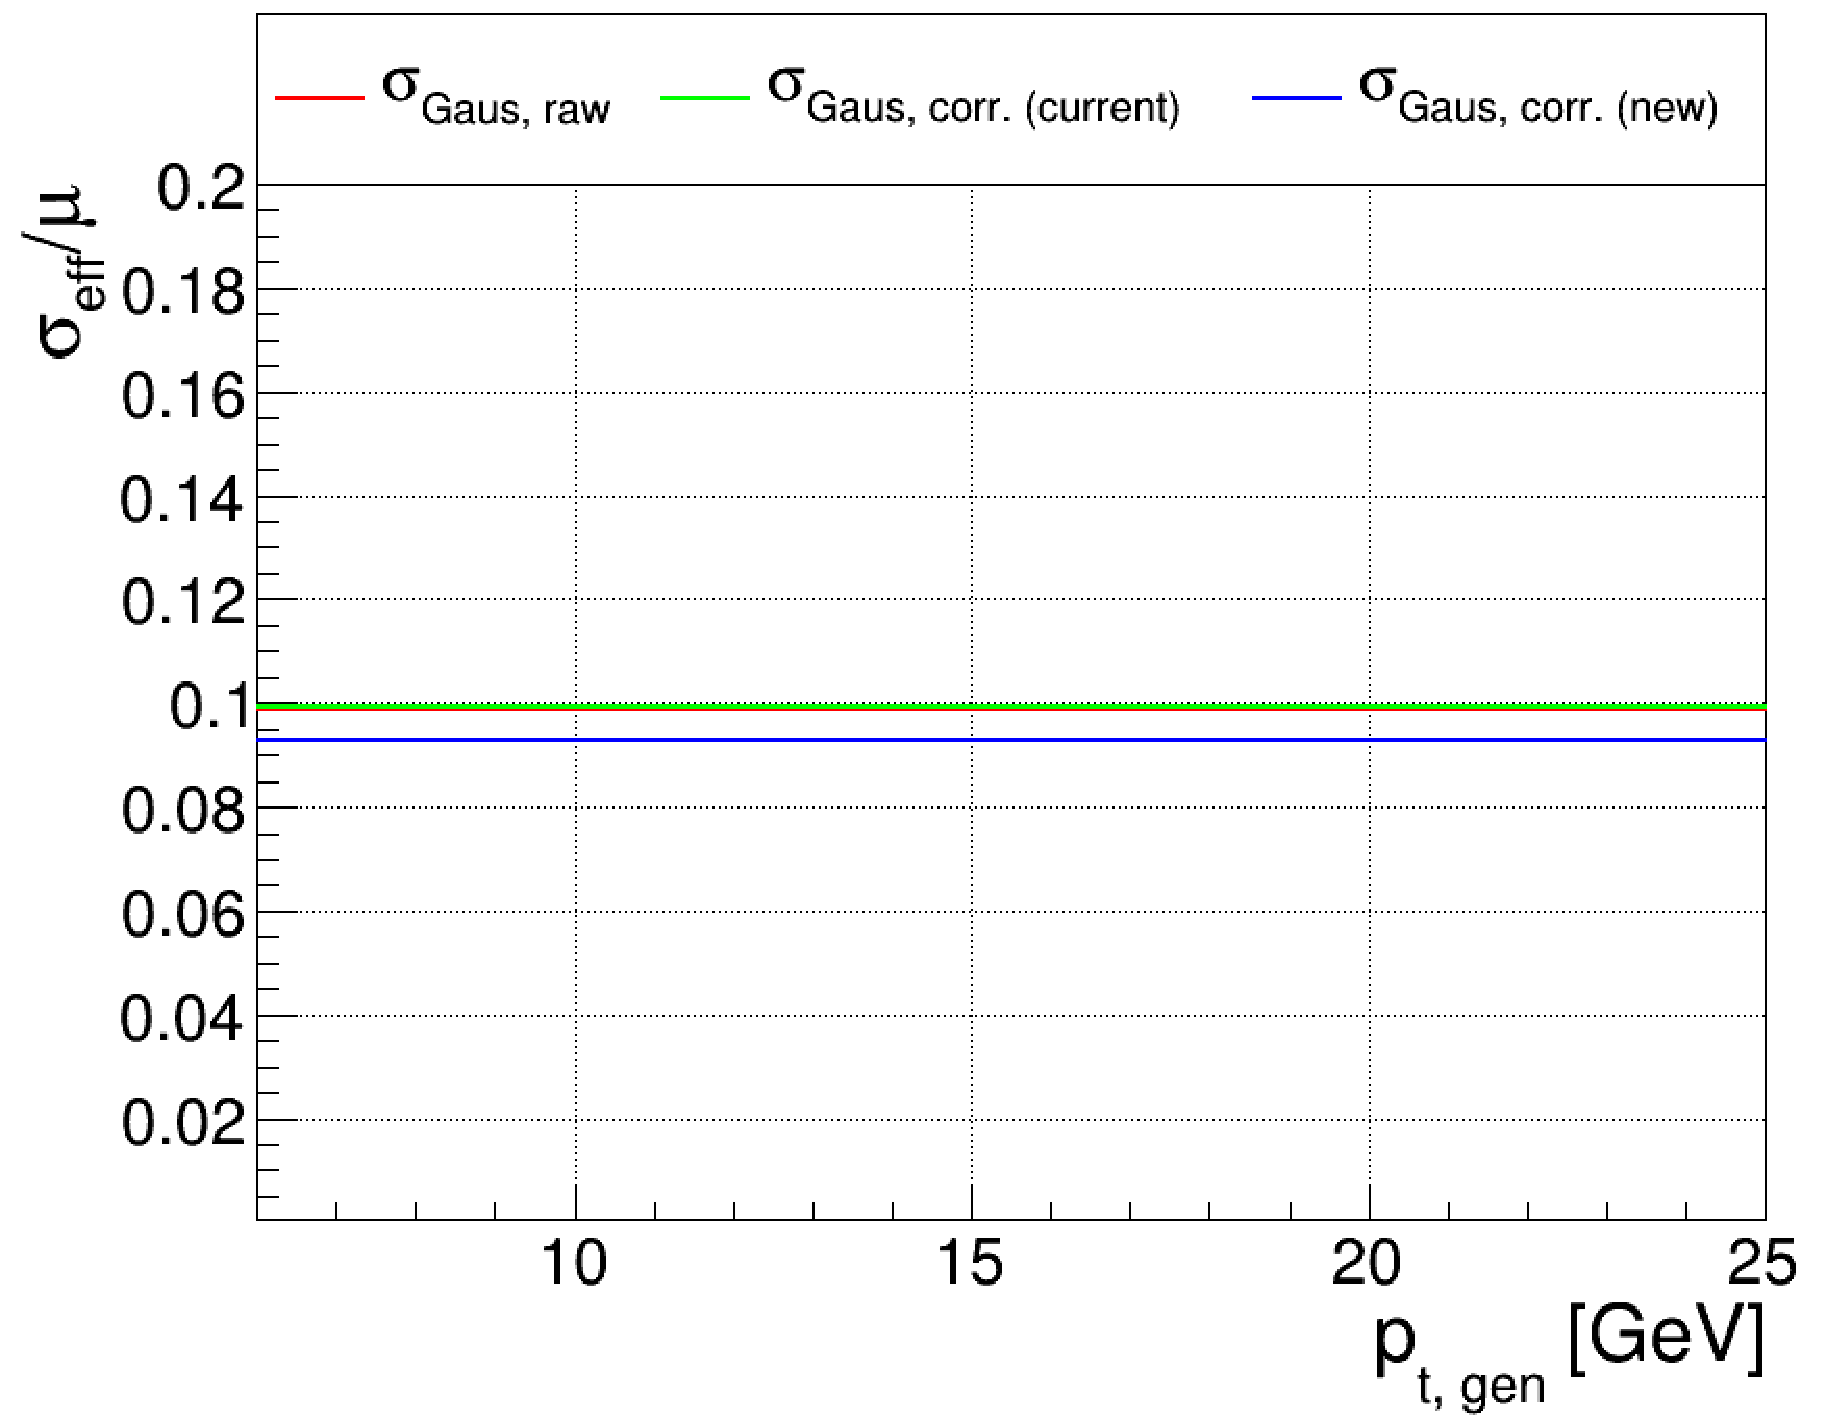
\includegraphics[width=0.495\textwidth]{./plots_pdf/ECAL_plots/plotsNoPU/EE/pdf/ZS/GENPT/EEZS_GENPT_0006_0025_EffSigmaOverBins.pdf}
%% %\caption{EE - ZS Readout pt 6-25}
%% %\end{figure}
%% %\begin{figure}
%% 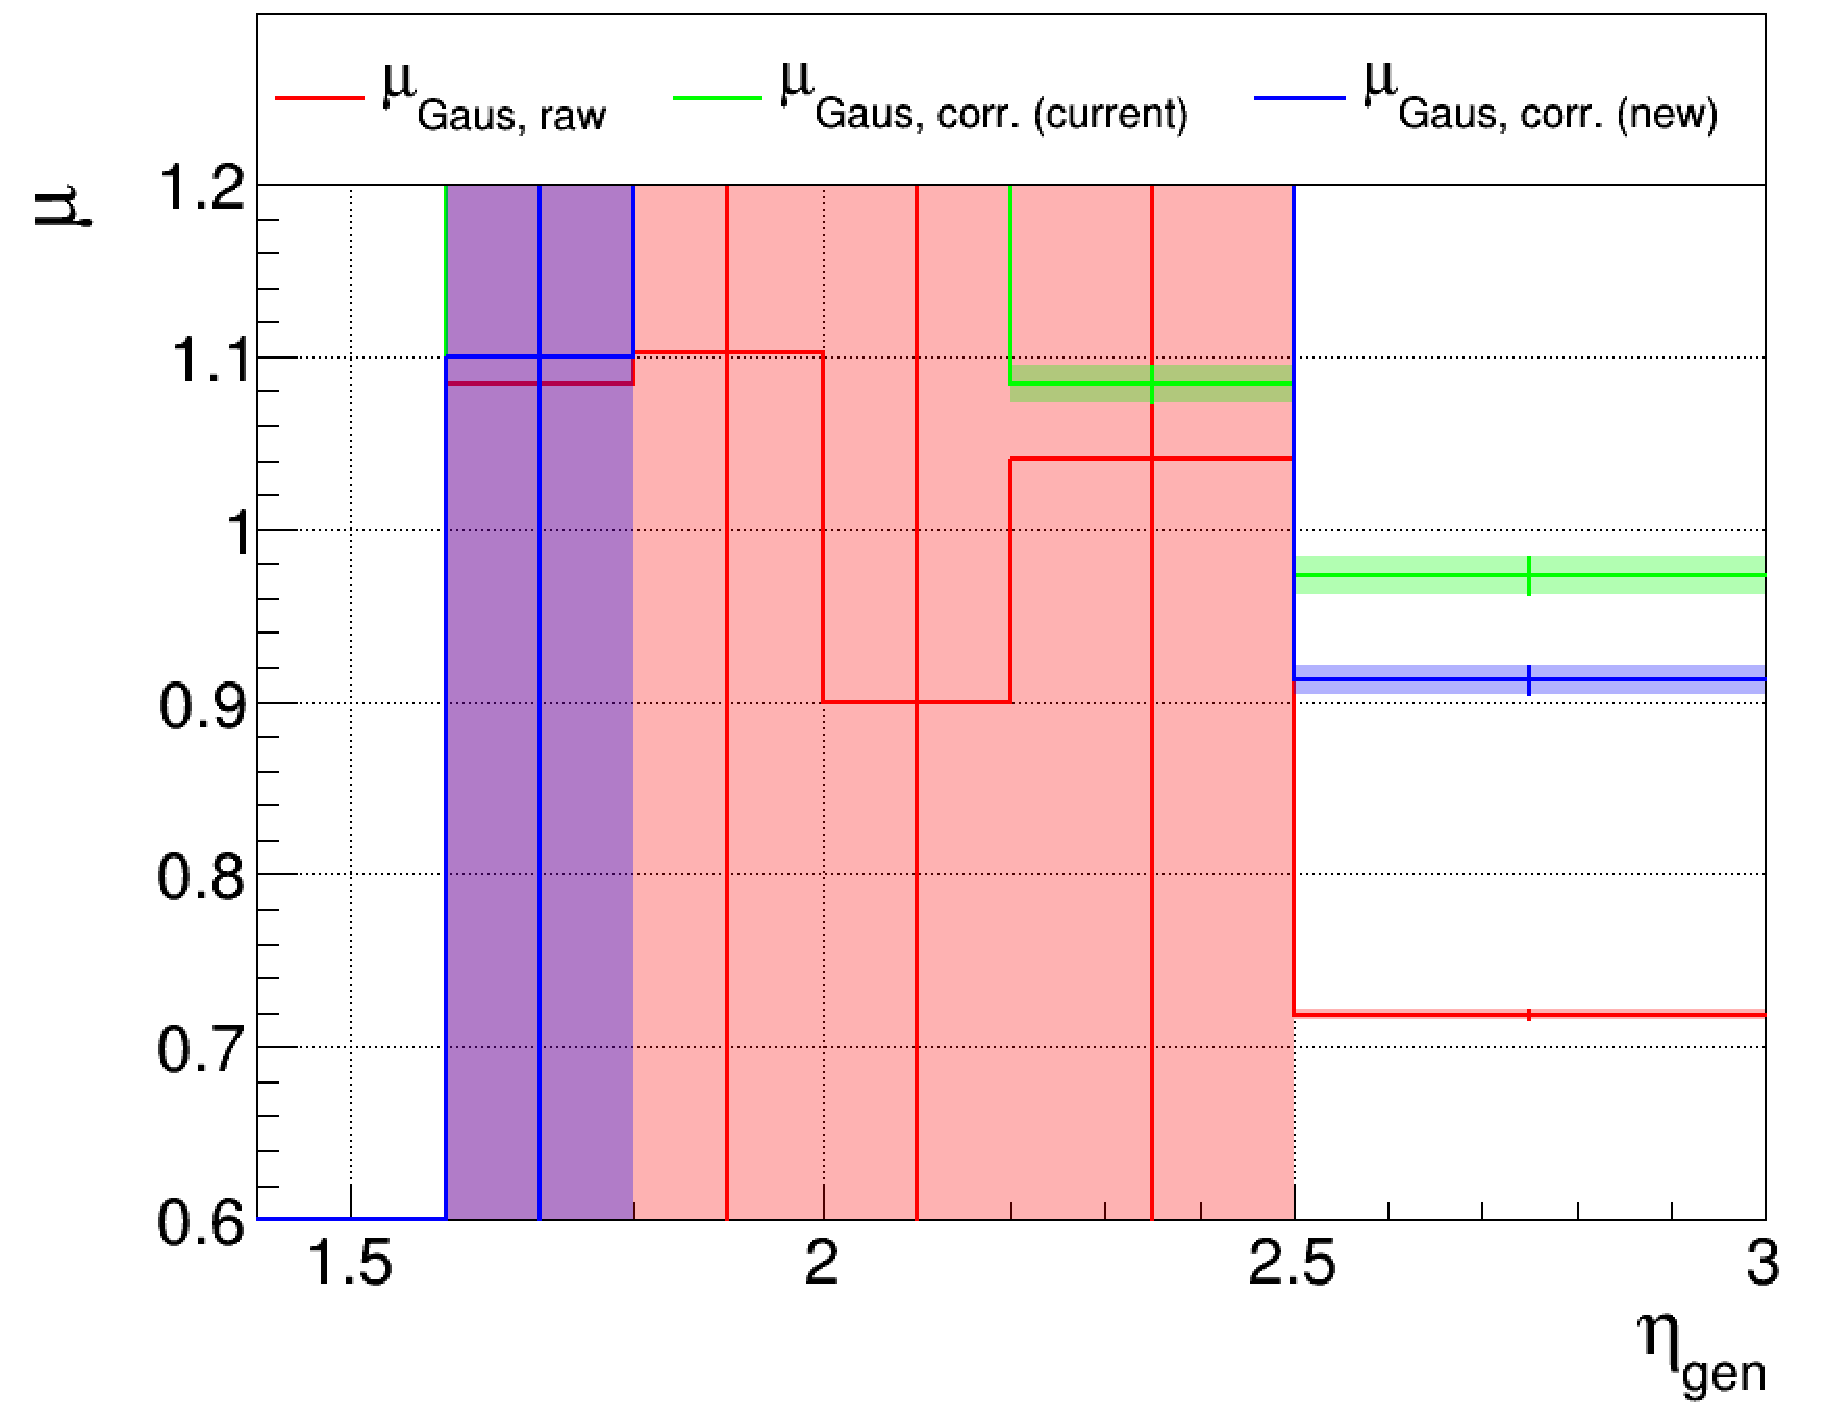
\includegraphics[width=0.495\textwidth]{./plots_pdf/ECAL_plots/plotsNoPU/EE/pdf/ZS/GENETA/EEZS_GENETA_0006_0025_MuOverBins.pdf}
%% %\includegraphics[width=0.495\textwidth]{./ECAL_plots/plotsNoPU/EE/pdf/ZS/GENETA/EEZS_GENETA_0006_0025_EffSigmaOverBins.pdf}
%% \caption{EE - ZS Readout \pt 6-25}
%% \end{figure}
